\begin{frame}
	\frametitle{Random variables}
	A variable quantity whose possible values depend, in random manner, on a set of random outcomes events\footnote{\href{https://en.wikipedia.org/wiki/Random_variable}{Wikipedia}}\vspace{1em}
	
	Every random variables is defined over \emph{probability space}: $(\Omega, \mathcal{F}, \mathcal{P})$ \footnote{Additional information can be found, among others, in \href{http://vfu.bg/en/e-Learning/Math--Bertsekas_Tsitsiklis_Introduction_to_probability.pdf}{D.P. Bertsekas and J.N. Tsitsiklis. Introduction to Probability}}\vspace{1em}
	
	Consider the toss of a coin
	\begin{itemize}
		\item $\Omega=\{H, T\}$ is the set of possible outcomes. In this case, head or tail
		\item $\mathcal{F}=\{\{\}, \{H\}, \{T\}, \{H,T\}\}$ is the set of events we consider
		\item $\mathcal{P}$ probability function. It associates elements of $\mathcal{F}$ with a probability value. For example $$\mathcal{P}(\{\})=0,\quad\mathcal{P}(\{H\})=0.5, \quad\mathcal{P}(\{T\})=0.5, \quad \mathcal{P}(\{H, T\})=1$$
	\end{itemize}
\end{frame}

\begin{frame}
	\frametitle{Moments}
	$X$ is a random variable , taking values in $\mathbb{R}$, and having probability density function $f(x)$
	\begin{itemize}
		\item Mean: $\mu=E[X]=\int_\mathbb{R} sf(s)ds$
		\item $n^{th}$ moment: $\int_\mathbb{R} s^nf(s)ds$ 
		\item $n^{th}$ central moment $E[(X-E[X])^n]=\int_\mathbb{R} (s-\mu)^nf(s)ds$
		\begin{itemize}
			\item Variance: second central moment $E[(X-E[X])^2]=\int_\mathbb{R} (s-\mu)^2f(s)ds$
		\end{itemize}
	\end{itemize}
	
	\vspace{1em}
	Some variables have moments on infinite value. For example \emph{heavy tailed distribution} \footnote{\href{https://en.wikipedia.org/wiki/Heavy-tailed_distribution}{\small{ Wikipedia. Heavy-tailed distribution}}} 
	$$f(x)=\left\{\begin{aligned}
					\frac{1}{x^2} && x \geq 1\\
					0&&\textrm{otherwise}
				   \end{aligned}
	\right.$$
\end{frame}

\begin{frame}
	\frametitle{Mean and mode (most likely outcome)}
	\emph{Mean} and \emph{mode} are different concept\vspace{0.5em}
	\begin{itemize}
		\item Mean: weighted sum of all of the possible outcomes
		\begin{itemize}
			\item Mean value could lie outside the set of possible outcomes
		\end{itemize}
		\item Mode: An outcome with the highest probability value
	\end{itemize}
	\vspace{0.5em}
	\begin{columns}
		\column{0.5\textwidth}
		$X$ is a random variable taking values
		\begin{itemize}
			\item 0 with probability 0.2 
			\item 1 with probability 0.8
		\end{itemize}
		\vspace*{0.5em}
	
	    Mean value: $\mu=0.2\cdot 0 + 0.8 \cdot 1=0.8$\\\vspace{0.5em}
	    
		Mode: $\argmax_{x\in\{0,1\}} p(x) \;=1$
		
		\column{0.4\textwidth}
		\begin{block}{Probability of $X$}
			\centering
			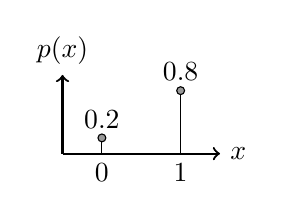
\begin{tikzpicture}
			%\draw[help lines, color=gray!30, dashed] (-4.9,-4.9) grid (4.9,4.9);
			\draw[->, thick] (-0.5,0)--(1.5,0) node[right]{$x$};
			\draw[->, thick] (-0.5,0)--(-0.5,1) node[above]{$p(x)$};
			\draw (0, 0) -- (0, 0.2) node [above] {$0.2$};
			\draw (1, 0) -- (1, 0.8) node [above] {$0.8$};
			\node [below] at (0,0) {0};
			\node [below] at (1,0) {1};
			\filldraw[fill=black!40, draw=black](0,0.2) circle (0.05cm);
			\filldraw[fill=black!40, draw=black](1,0.8) circle (0.05cm);
			\end{tikzpicture}
		\end{block}
	\end{columns}
	
	
	%Under certain assumptions (e.g., Ergodicity) the average of 
	
	\takeaway{\bf{The mean value is not even an element of the possible outcomes}}
\end{frame}
\begin{frame}
	\frametitle{Sum of independent random variable}
	\onslide<1->The distribution of the sum of two random variables must always be carefully computed\vspace{0.5em}
	\begin{columns}\onslide<1->
		\column{0.5\textwidth}
		\begin{itemize}
			\item <1->$X$ uniformly distributed between 0 and 1%, $X\sim\mathcal{U}(0, 1)$
			\item <1->$Y$ uniformly distributed between 0 and 1
			\item <1->$Z=X+Y$ \emph{is not} uniformly distributed between 0 and 1
			\item <2-> The distribution of $Z$ depends on the joint distribution of $X$ and $Y$
			\item <3-> If $X$ and $Y$ are independent variables, then $Z$ has a triangular distribution\\
			\begin{itemize}
				\item $X$ and $Y$ are independent if
				for all $x$ and $y$ $$P(X\leq x,Y\leq y)=P(X\leq x)\cdot P(Y \leq y)$$	
			\end{itemize}	
		\end{itemize}
	
		\column{0.46\textwidth}
		\begin{block}{Probability density functions}
			\onslide<1->{
			\begin{tikzpicture}
				\draw[->] (-0.5,0)--(1.5,0) node[right]{$x$};
				\draw[->] (-0.5,0)--(-0.5,1.5) node[above]{$p(x)$};
				\draw[very thin, dashed] (-0.5, 1)node[left] {1} -- (0, 1);
				\draw[thin](0, 0) node[below] {0}-- (0, 1);
				\draw[thick] (0, 1) -- (1, 1); 
				\draw[thin] (1, 0)node[below] {1} -- (1, 1);
			\end{tikzpicture}}
			\onslide<3->{
			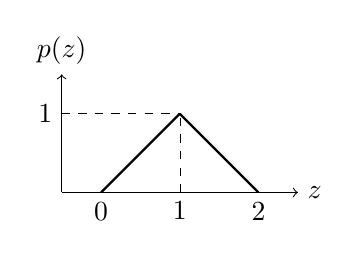
\begin{tikzpicture}
			\draw[->] (-0.5,0)--(2.5,0) node[right]{$z$};
			\draw[->] (-0.5,0)--(-0.5,1.5) node[above]{$p(z)$};
			\draw[very thin, dashed] (-0.5, 1)node[left] {1} -- (1, 1);
			\draw[thick](0, 0) node[below] {0}-- (1, 1);
			\draw[very thin, dashed] (1, 0)node[below]{1} -- (1, 1); 
			\draw[thick] (2, 0)node[below] {2} -- (1, 1);
			\end{tikzpicture}}
		\end{block}
	\end{columns}
\end{frame}
\begin{frame}
	\frametitle{Sum of variables normally distributed random variables}
	The Gaussian distribution is also called \emph{Normal} distribution and is denoted with the symbol $\mathcal{N}$\vspace{0.5em}
	
	\begin{itemize}
		\item The probability density function of a normally distributed random variable $X$ is
		$$f_X(x;\mu,\sigma)=\frac{1}{\sigma\sqrt{2\pi}}e^{-\frac{(x-\mu)^s}{2\sigma^2}}$$
		\item <2-> If $X\sim\mathcal{N}(\mu_x, \sigma_x^2)$ and $Y\sim\mathcal{N}(\mu_y, \sigma_y^2)$ and are independent, then
		\item <2-> $Z=X+Y$ is also normally distributed;\vspace{1em} $Z\sim\mathcal{N}(\mu_x+\mu_y, \sigma_x^2+\sigma_y^2)$
		%\item <2-> If $\alpha$ is a non-zero constant, then $\alpha Z$ is normally distributed
		%\begin{itemize}
		%	\item mean: $\alpha \mu_z$, variance: $\alpha^2\sigma_z^2$
		%\end{itemize}
	
		\item <3-> If $\bm{Z}$  has a multivariate normal distribution with mean $\bm{\mu}_z$ and covariance $L=E[(Z-\bm{\mu}_z)(Z-\bm{\mu}_z)^T]$
		and $A$ is a matrix, then
		\item <3-> The variable $\bm{S}=A\bm{Z}$ is normally distributed with mean $A \bm{\mu}_z$ and covariance matrix is $ALA^T$
	\end{itemize} 
\onslide<2>{
\takeaway{\large Note however that $X\cdot Y$ is \emph{not} normally distributed}}
\end{frame}

\section{Random variables and dynamic systems}
\separatorslide

\begin{frame}
	\frametitle{Gaussian distributions and linear systems}
	Assume 
	\begin{columns}
		\column{0.6\textwidth}
		\begin{itemize}
			\item $X(0)$ is normally distributed, $X(0)\sim\mathcal{N}(\mu_0, \sigma_0^2)$
			\item $W(k)$ is normally distributed, $W(k)\sim\mathcal{N}(\mu_{w,k}, \sigma_{w,k}^2)$
			\item $X(0)$ and $W(k)$ are independent for all $k$
			\item for $k\geq0$ the following recursive equation holds: $X(k+1) =X(k) + W(k)$
		\end{itemize}	
		\column{0.4\textwidth}
		\begin{block}{Graphical representation}
			\begin{tikzpicture}
			\node(X0){$X(0)$};
			\node[above=1em of X0](W0){$W(0)$};
			\node[right=1em of X0](sum1){$+$};
			\node[right=1em of sum1](X1){$X(1)$};
			\node[above=1.2em of X1](W1){$W(1)$};
			\node[right=1em of X1](sum2){$+$};
			\node[right=1em of sum2](X3){$\cdots$};
			\draw[->] (W0) to (sum1);
			\draw[->] (X0) to (sum1);
			\draw[->] (sum1) to (X1);
			\draw[->] (W1) to (sum2);
			\draw[->] (X1) to (sum2);
			\draw[->] (sum2) to (X3);
			\end{tikzpicture}		
		\end{block}
	\end{columns}
	
	\vspace*{0.5em}

	\onslide<1-> What is the distribution of $X(1)$ ?
	\begin{itemize}\onslide<2->
		\item $X(1)$ is normally distributed (sum of two independent Gaussian variables)
		\item Mean $\mu_1=\mu_0+\mu_{w,0}$, variance $\sigma_1^2 = \sigma_0^2 + \sigma_{w,0}^2$
	\end{itemize}

	\vspace*{0.5em}
	\onslide<2-> What is the distribution of $X(k)$ ?
	\begin{itemize}\onslide<3->
		\item $X(k)$ is Gaussian distributed% (sum of independent Gaussian variables)
		\item Mean $\mu_k=\mu_0+\sum_{j=0}^{k-1}\mu_{w,j}$, variance $\sigma_k^2=\sigma_0^2 + \sum_{j=0}^{k-1}\sigma_{w,j}^2$
	\end{itemize}
\end{frame}

\begin{frame}
	\frametitle{Non Gaussian distributions and linear systems}
	Assume 
	\begin{columns}
		\column{0.6\textwidth}
		\begin{itemize}
			\item $X(0)$ is uniformly distributed, $X(0)\sim\mathcal{U}(0, 1)$
			\item $W(k)$ is uniformly distributed, $W(k)\sim\mathcal{U}(0, 1)$
			\item $X(0)$ and $W(k)$ are independent for all $k$
			\item for $k\geq0$ the following recursive equation holds: $X(k+1) =X(k) + W(k)$
		\end{itemize}	
		\column{0.4\textwidth}
		\begin{block}{Graphical representation}
			\begin{tikzpicture}
			\node(X0){$X(0)$};
			\node[above=1em of X0](W0){$W(0)$};
			\node[right=1em of X0](sum1){$+$};
			\node[right=1em of sum1](X1){$X(1)$};
			\node[above=1.2em of X1](W1){$W(1)$};
			\node[right=1em of X1](sum2){$+$};
			\node[right=1em of sum2](X3){$\cdots$};
			\draw[->] (W0) to (sum1);
			\draw[->] (X0) to (sum1);
			\draw[->] (sum1) to (X1);
			\draw[->] (W1) to (sum2);
			\draw[->] (X1) to (sum2);
			\draw[->] (sum2) to (X3);
			\end{tikzpicture}		
		\end{block}
	\end{columns}
	
	\vspace*{0.5em}
	
	\onslide<2-> What is the distribution of $X(1)$ ?
	\begin{itemize}\onslide<3->
		\item $X(1)$ has a triangular distribution
		\item Mean $\mu_1=\mu_0+\mu_{w,0}$, variance $\sigma_1^2 = \sigma_0^2 + \sigma_{w,0}^2\;$\footnote{\href{http://eli.thegreenplace.net/2009/01/07/variance-of-the-sum-of-independent-variables}{See also here}}
	\end{itemize}
	
	\vspace*{0.5em}
	\onslide<4-> What is the distribution of $X(k)$ ?
	\begin{itemize}\onslide<4->
		\item The distribution of $X(k)$ depends on the distribution of $X(k-1)$ and of $W(k-1)$
		\item Mean $\mu_k=\mu_0+\sum_{j=0}^{k-1}\mu_{w,j}$, variance $\sigma_k^2=\sigma_0^2 + \sum_{j=0}^{k-1}\sigma_{w,j}^2$
		
	\end{itemize}
\end{frame}

\begin{frame}
	\frametitle{Gaussian distributions and non linear systems}
	Assume 
	\begin{columns}
		\column{0.6\textwidth}
		\begin{itemize}
			\item $X(0)$ is normally distributed $X(0)\sim\mathcal{N}(0, 1)$
			\item $W(k)$ is normally distributed $W(k)\sim\mathcal{N}(0, 1)$
			\item $X(0)$ and $W(k)$ are independent for all $k$
			\item for $k\geq0$ we have $X(k+1) =X^2(k) + W(k)$
		\end{itemize}	
		\column{0.4\textwidth}
		\begin{block}{Graphical representation}
			\begin{tikzpicture}
			\node(X0){$X(0)$};
			\node[above=1em of X0](W0){$W(0)$};
			\node[right=1em of X0](sum1){$+$};
			\node[right=1em of sum1](X1){$X(1)$};
			\node[above=1.2em of X1](W1){$W(1)$};
			\node[right=1em of X1](sum2){$+$};
			\node[right=1em of sum2](X3){$\cdots$};
			\draw[->] (W0) to (sum1);
			\draw[->] (X0) to (sum1);
			\draw[->] (sum1) to (X1);
			\draw[->] (W1) to (sum2);
			\draw[->] (X1) to (sum2);
			\draw[->] (sum2) to (X3);
			\end{tikzpicture}		
		\end{block}
	\end{columns}
	
	\vspace*{0.5em}
	
	\onslide<2-> What is the distribution of $X(1)$ ?
	\begin{itemize}\onslide<3->
		\item $X(1)$ is not normally distributed.
		\item Mean $\mu_1=E[X(0)^2]+\mu_{w,0}$
		\item Variance $\sigma_1^2=var(X(0))+\sigma_{w,0}^2$
	\end{itemize}
\end{frame}

\begin{frame}
	\frametitle{Few remarks}
	\begin{itemize}
		\setlength\itemsep{2em}
		\item Mean of the sum is always equal to the sum of the means (linear operator)
		\item If two random variables are independent, then the variance of the sum is equal to the sum of the variances 
		%\item Variables $X(k)$ are normally distributed for all $k\geq0$ \emph{only} in the case of linear systems and if the variables $w(k)$ are normally distributed
		\item The knowledge of mean and variance rarely completely characterize the distribution of a random variable
	\end{itemize}  
\end{frame}

\section{Marginal and conditional density functions}
\separatorslide
\begin{frame}
	\frametitle{Marginal and conditional density functions}
	Assume $X$ and $Y$ are two random variables taking values in the interval $[0, 1]$\vspace{0.5em}\\
	and $f_{X,Y}(x,y)$ is the joint probability density function of $X$ and $Y$\vspace{0.5em}
	%The following probabilities can be computed from the joint distribution of $X$ and $Y$
 	\begin{itemize}%\setlength\itemsep{0.5em}
 		\item <1-> Marginal probability density functions are given by
 		$$f_{X}(x)=\int_0^1f_{X,Y}(x,z) dz\;, \qquad f_{Y}(y)=\int_0^1f_{X,Y}(z,y) dz$$
 		
 		%Probability of $X$ taking value $x$ independently of the value taken by $Y$ 
 		%\item Marginal probability density function
 		%Probability of $X$ taking value $x$ independently of the value taken by $Y$ 
 		%\item <1-> %Probability of $Y$ taking value $y$ independently of the value taken by $X$ 
 		%$P(Y\leq y)=\int_0^y\int_0^1 P(X=z, Y=y) dz$ (Marginal distribution)
 		%\item <2-> %Probability of $Y$ taking value $y$ once we know that $X$ has value $x$
 		% $P(Y\leq y|X=x)=\int_0^y \frac{P(X=x, Y=y)}{P(X=x)}$ (Conditional distribution)
 		%\item <2->Probability of $X$ taking value $x$ once we know that $Y$ has value $y$ %$P(X=x|Y=y)=\frac{P(X=x, Y=y)}{P(Y=y)}$ (Conditional distribution)
 		
 		\item <2-> Conditional probability density function: $f_{X|Y}(x;y)=\frac{f_{X,Y}(x,y)}{f_{Y}(y)},$ if $f_Y(x)>0$ 
 		\item <3-> Conditional mean and variance of $X$ given $Y$ 
		$$E[X|Y=y]\!=\int_0^1\!\! zf_{X|Y}(z;y)dz,\quad var(X|Y=y)\!=\int_0^1 \!\!(z-E[X|Y=y])^2f_{X|Y}(z;y)dz$$
 	\end{itemize}
 	
\end{frame}

\begin{frame}
	\frametitle{Conditional distribution and expected conditional risk}
	Consider the case of estimating the value of a variable $X$ from its measurement $Y$
	\begin{itemize}
		\item For example $Y=X+W$, where $W$ is random noise independent of $X$
		\item The conditional distribution of $X|Y$ provides information about the probability of different values of $X$ given that $Y=y$
		\item <3-> For selecting a best value, we need a cost function, e.g., the \emph{expected conditional risk}
		$$R(t,y)=E[c(t-X)|Y=y]=\int_{\mathbb{R}}c(t-z)f_{X|Y}(z;y)dz$$
	\end{itemize}
	
	\onslide <3->If
	\begin{itemize}
		\item $c(t-x)$ is symmetric, e.g., $c(z-x)=(z-x)^2$ and
		\item the conditional density function $f_{X|Y}(z;y)$ is symmetric around $E(X|Y=y)$,
	\end{itemize}
	then
	\begin{itemize}
		\item the minimum of $R(t,y)$ does not depends on the specific cost function $c(t-X)$
		\item \emph{the minimum of $R(t,y)$ is given by $E[X|Y=y]$}
	\end{itemize}
%\onslide<2->
%\takeaway{Under these assumption, the best estimate of $X$ given $Y=y$ is $E[X|Y=y]$}
\onslide<2>\takeaway{\bf{How could we select a best \emph{value} for $X$?}}
\end{frame}

\begin{frame}
	\frametitle{The Maximum a posteriori estimator}
	Another approach for selecting a best value for the estimation of $X$ given $Y=y$ could be to take the maximum of $f_{X|Y}(z;y)$ \vspace{2em}
	\begin{itemize}
		\item We can define $$\hat{x}(y)=\argmax_{z\in\mathbb{R}}f_{X|Y}(z;y)$$
		\item This estimator is called \emph{Maximum a posteriori} (MAP) 
	\end{itemize}
	\begin{itemize}
		\item For unimodal and symmetric distributions, e.g., Gaussian distribution, then MAP estimator and the expected conditional value estimator coincide
	\end{itemize}
\takeaway{In general, MAP and the expected conditional value are different}	 
\end{frame}

%\begin{frame}
%	\frametitle{Some properties of the conditional expectation}
%	Assumptions:
%	\begin{itemize}
%		\item $c(z-x)$ is symmetric, e.g., $c(z-x)=(z-x)^2$
%		\item the conditional distribution of $(X|Y=y)$ is symmetric around $E(X|Y=y)$
%	\end{itemize}\vspace{1em}
%	then
%	\begin{itemize}
%		\item the minimum of $R(z,y)$ does not depends on the specific cost function $c(z-X)$
%		\item the minimum of $R(z,y)$ is given by $E[X|Y=y]$
%	\end{itemize}\vspace{1.5 em}
%		
%	\takeaway{Under these assumptions mean and mode of the conditional distribution coincide}
%\end{frame}